\chapter{Réalisations}
Dans la section précédente, j'ai déjà mentionné que mon stage était principalement axé sur \texttt{PowerEye}. Dans cette section, je détaillerai mes réalisations, en commençant par l'architecture globale, puis les modules individuels, et enfin certaines fonctionnalités en dehors du corps principal du logiciel.
\section{Architecture globale de PowerEye}
Dans cette partie, je présenterai la composition du \texttt{PowerEye} en termes d'architecture global, y compris le choix de modèle de conception, la construction de la structure de données de l'interface et l'apparence de l'interface. De cette façon, vous pouvez d'abord avoir un concept général du \texttt{PowerEye}, et comprendre plus facilement la conception du chaque module dans les parties suivant.
\subsection{Modèle de conception}
Le choix du modèle de conception influe grandement sur la manière de développer le programme. Au début du développement du \texttt{PowerEye}, j'ai choisi MVVM comme modèle de conception.
\subsubsection{Présentation du MVVM}
Il existe trois composants principaux dans le modèle MVVM : le modèle, la vue et le modèle de vue. Chacun sert un objectif distinct. La vue est chargée de définir la structure, la disposition et l’apparence de ce que l’utilisateur voit à l’écran. Le modèle de vue implémente des propriétés et des commandes avec lesquelles la vue peut effectuer une liaison aux données. Les classes de modèle sont des classes non visuelles qui encapsulent les données de l’application. Ainsi, le modèle peut être considéré comme une représentation du modèle de domaine de l’application, qui comprend généralement un modèle de données avec une logique métier et une logique de validation. \\
\subsubsection{Application pratique}
Au début de la conception du \texttt{PowerEye}, nous avons décidé d'utiliser \gls{WPF} pour le développement du logiciel. Et \gls{WPF} offre une fonctionalité très important, à savoir la liason de données. C'est le processus qui établit une connexion entre l’IU du logiciel et les données affichées. Si la liaison est correctement paramétrée et si les données fournissent les notifications appropriées, lorsque les données changent de valeur, les éléments qui sont liés aux données reflètent automatiquement ces changements. Comme le montre la figure ci-dessous, lorsque la source de la liaison de données est modifiée, la valeur target de la liaison est modifiée en conséquence. En pratique, nous pouvons lier les propriétés des contrôles au modèle des données.
\begin{figure}[H]
    \centering
    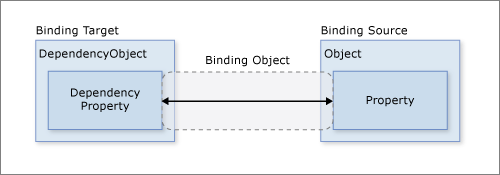
\includegraphics[height=3cm]{ressources/images/basic-data-binding-diagram.png}
    \caption{La liaison de données}
\end{figure}

Grâce à cette caractéristique, il est facile d'utiliser les changements apportés à la partie modèle de MVVM pour conduire des changements dans l'affichage de l'interface. Plus précisément, lors du développement du \texttt{PowerEye}, j'utilise des informations de données telles que les chemins sélectionnés et les fichers ouverts comme la partie modèle. Et le modèle de vue contient la partie modèle et les fonctions de contrôle des événements. Enfin, l'apparence de l'interface apparaît comme la vue. En outre, pour rendre la structure global plus claire, j'ai établi une distinction entre la couche de présentation et la couche d'applications.
\begin{figure}[H]
    \centering
    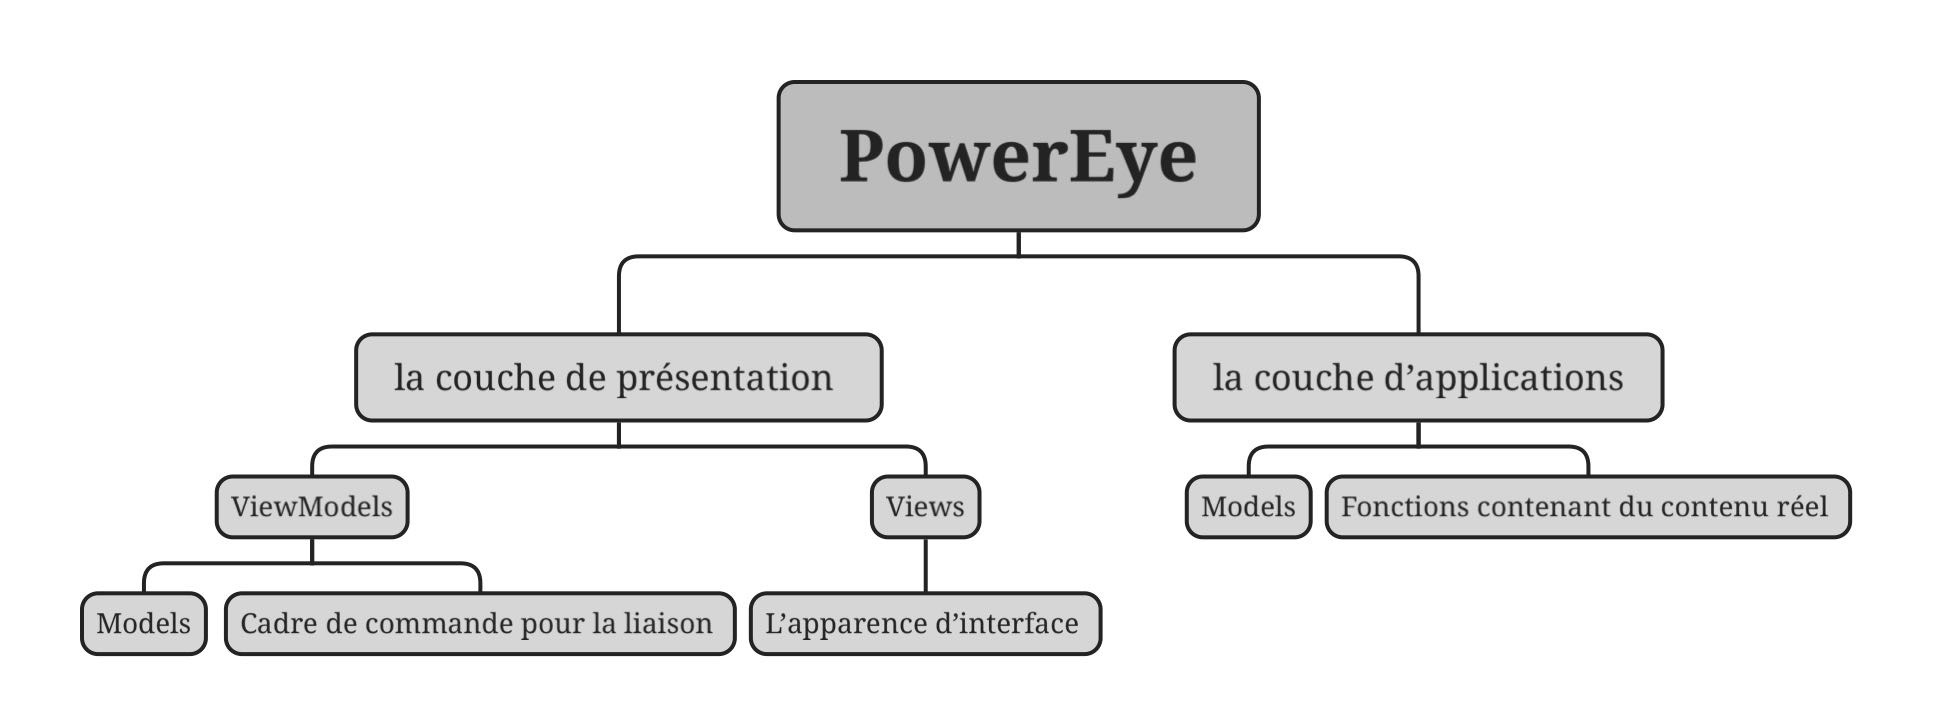
\includegraphics[height=5cm]{ressources/images/PowerEye_Structure.jpg}
    \caption{La structure globale du PowerEye}
\end{figure}

\subsubsection{Avantages de ce choix}
L'utilisation de ce modèle de conception facilite grandement l'ensemble du processus de développement. Premièrement, il sépare le développement de l'apparence de l'interface de l'ensemble. Une fois l'apparence de l'interface développée, l'adaptation des données peut être réalisée en modifiant simplement la source de la liaison de données. De plus, nous pouvons réutiliser le modèle de vue pour des interfaces similaires. Enfin, comme la couche d'application est séparée, il est possible d'appeler directement des fonctions qu'elle contient pour tester.

\subsection{Structure des données}
Les données font partie du modèle dans le cadre de MVVM, je les ai également conçu pour répondre aux besoins. Pour chaque module, j'ai créé une sous-classe avec une liste pour stocker les instances qui ont été créées. Afin que les différentes interfaces d'un même module puissent être enregistrées dans la même liste, j'ai créé une classe de base. Enfin, les classes de chaque interface héritent simplement de la classe de base et modifiée différemment en fonction des besoins. En outre, la classe de base doit hériter de la classe \texttt{BindingBase} pour implémenter la fonctionnalité de notification de l'interface lorsqu'une propriété est changée. Et voici un aperçu de la structure des données.

\begin{figure}[H]
    \centering
    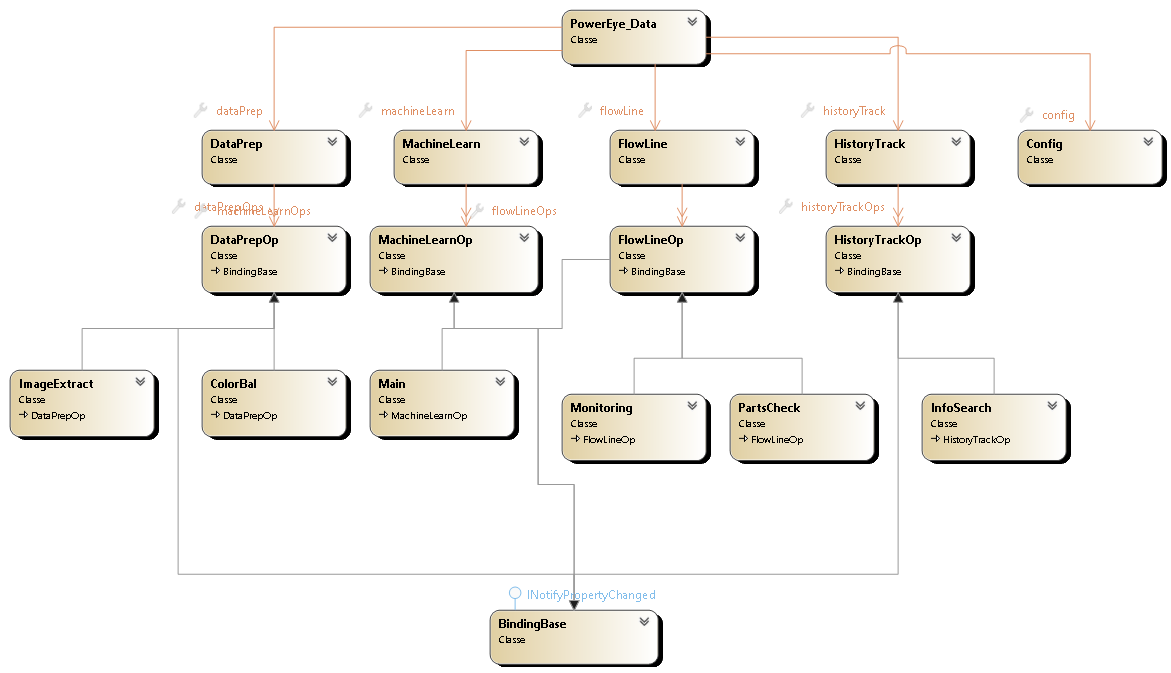
\includegraphics[height=9cm]{ressources/images/PowerEye_Data.png}
    \caption{La structure des données du PowerEye}
\end{figure}
\subsection{Disposition de l'interface graphique}
Après avoir présenté la partie du modèle, j'aimerais expliquer la conception de la disposition de l'interface graphique, c'est-à-dire la partie concernant la vue dans le cadre de MVVM. La \hyperref[fig:target]{\textsc{figure 2}} montre le style d'interface du \texttt{PowerEye}, qui semble se composer de trois parties. Mais ce n'est pas vraiment ce que j'ai fait avec l'interface au début. Au départ, j'ai choisi le \texttt{Tabcontrol} pour séparer les modules et les développer à partir de là. L'interface conçue à ce moment-là est illustrée ci-dessous.
\begin{figure}[H]
    \centering
    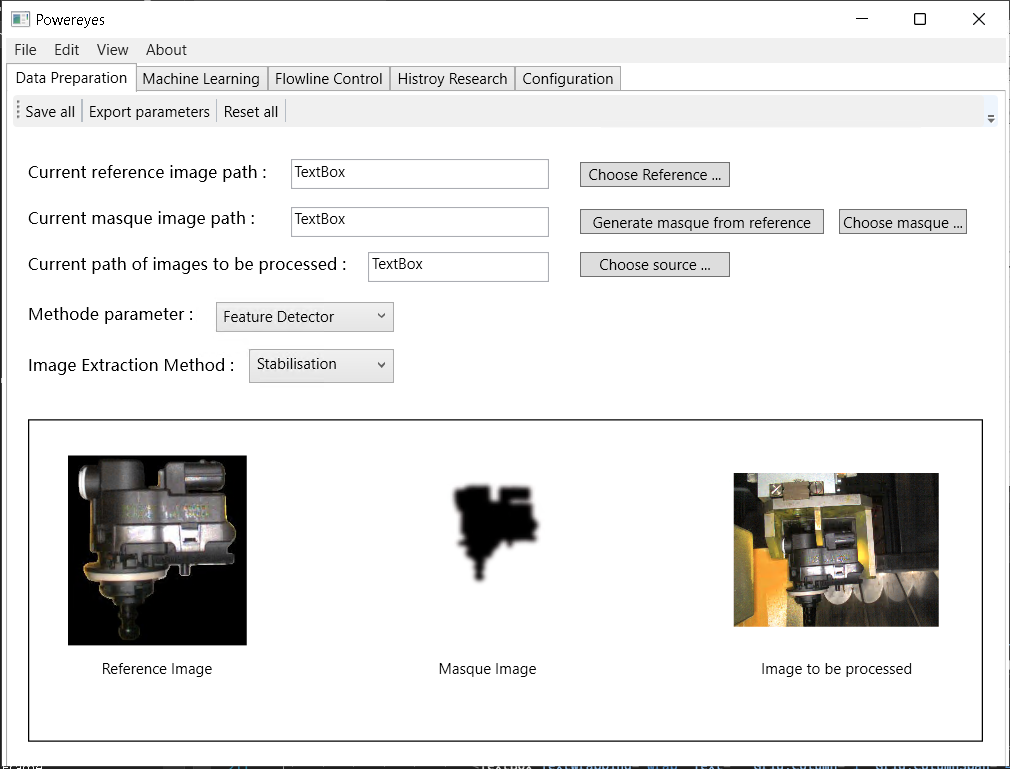
\includegraphics[height=8cm]{ressources/images/Interface_original.png}
    \caption{La Conception initiale de l'interface}
\end{figure}

Cependant, le problème est double: d'une part, chaque module n'a pas nécessairement une seule fonction, et les combiner dans une interface unique aurait l'air encombré. D'autre part, avec cette approche, le développement de toutes les interfaces des modules se fait dans le même ficher, ce qui réduit la lisibilité du code.

J'ai donc finalement choisi d'abandonner cette solution et d'utiliser 
\texttt{Contentcontrol} pour la disposition de l'interface. Plus précisément, j'ai divisé l'interface globale en trois parties: la barre des modules, la barre des fonctions et la fenêtre principale. En sélectionnant le module, différentes barres de fonctions s'affichent, puis la fenêtre principale est affichée en cas de sélection de la fonction. Et grâce à la caractéristique du \texttt{Contentcontrol}, nous pouvons injecter l'interface en tant que contrôle, ce qui permet le développement indépendant des différentes parties. La disposition finale de l'interface est illustrée ci-dessous.
\begin{figure}[H]
    \centering
    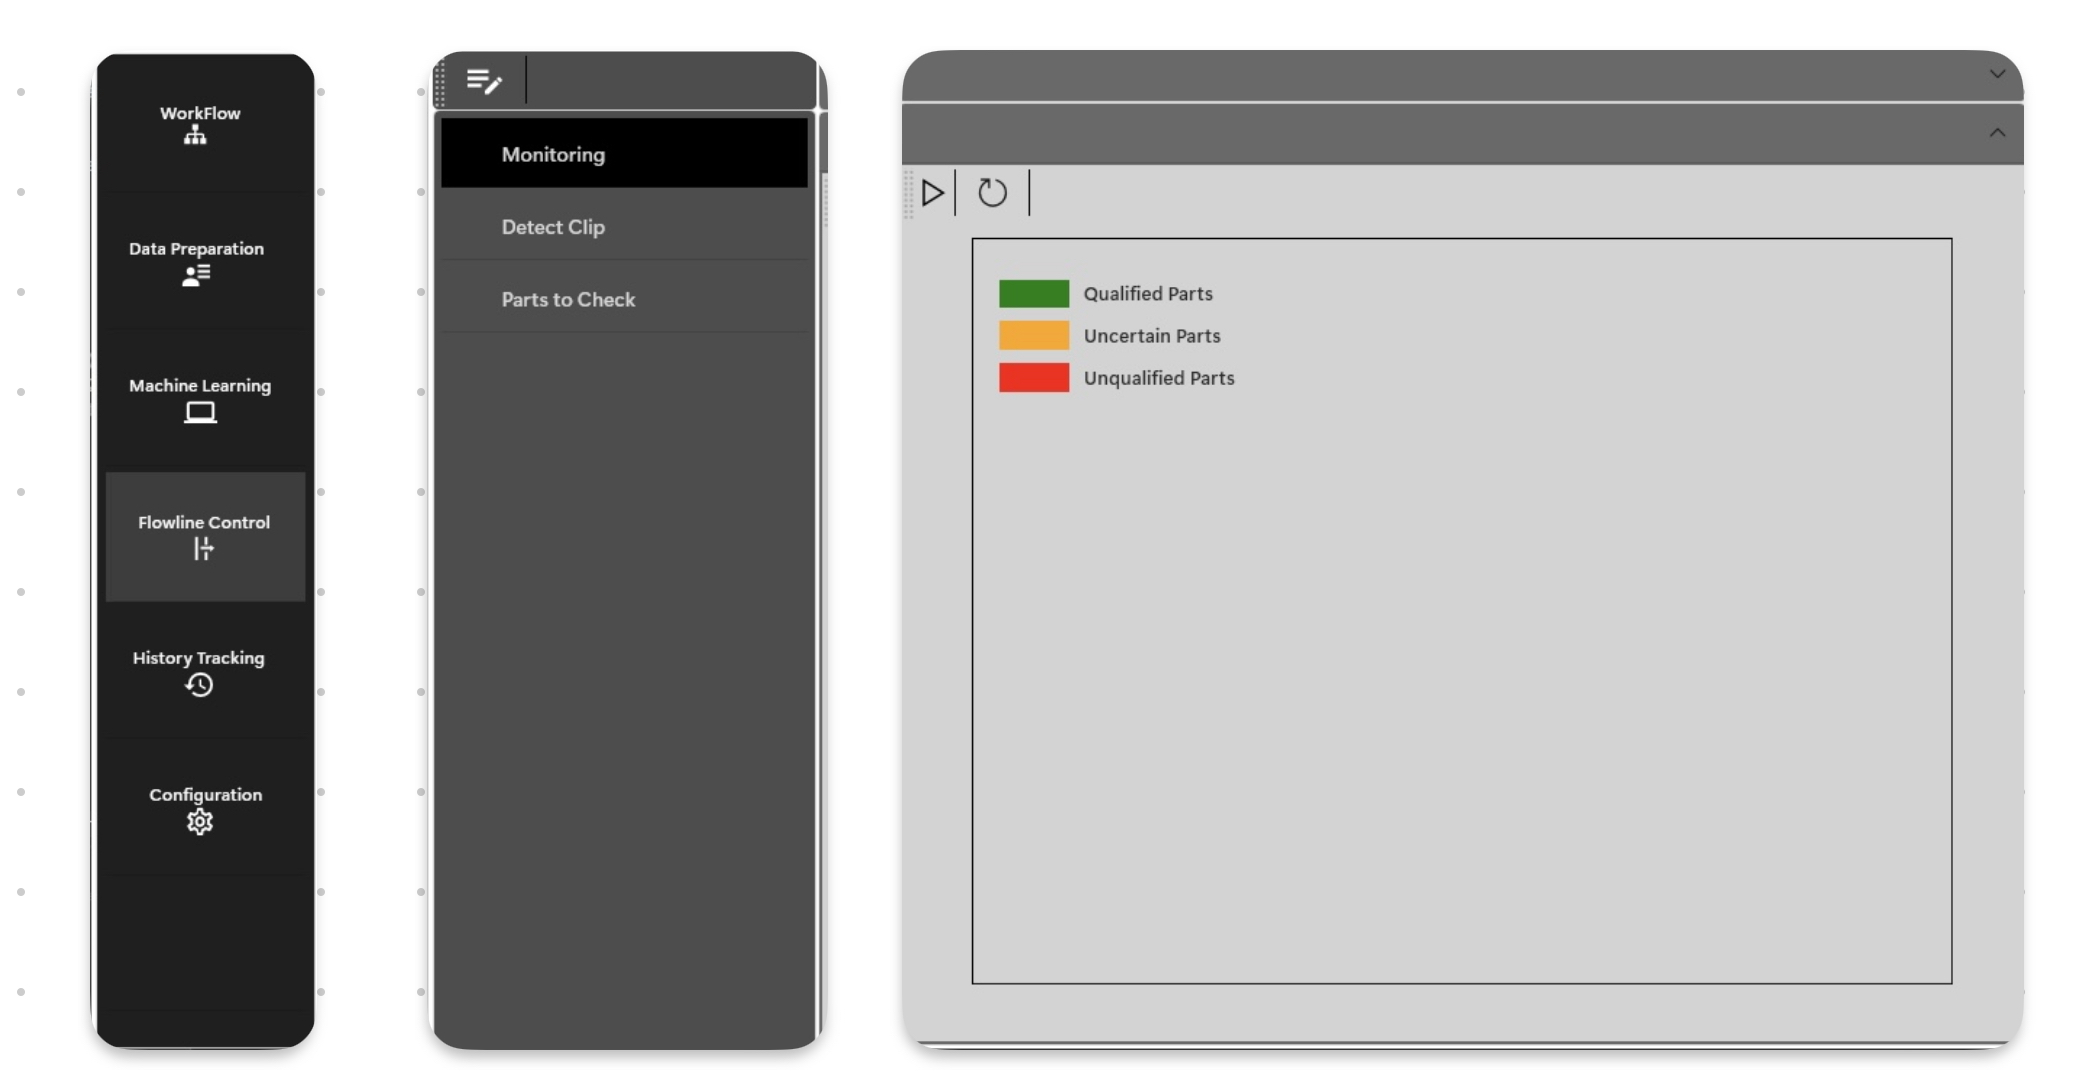
\includegraphics[height=8cm]{ressources/images/PowerEye_Disposition.jpg}
    \caption{ La disposition finale de l’interface}
\end{figure}

Dans la partie de la fenêtre principale, compte tenu du fait que la réalisation de nombreuses fonctions nécessite la sélection du chemin d'accès au ficher et d'autres configurations, j'ai également fait la conception correspondante. L'\texttt{Expander} est utilisé pour diviser la fenêtre en deux parties, la partie supérieure pour les choix de configuration et la partie inférieure pour les fonctionnalités. La figure suivant montre spécifiquement la fenêtre principale. 
\begin{figure}[H]
    \centering
    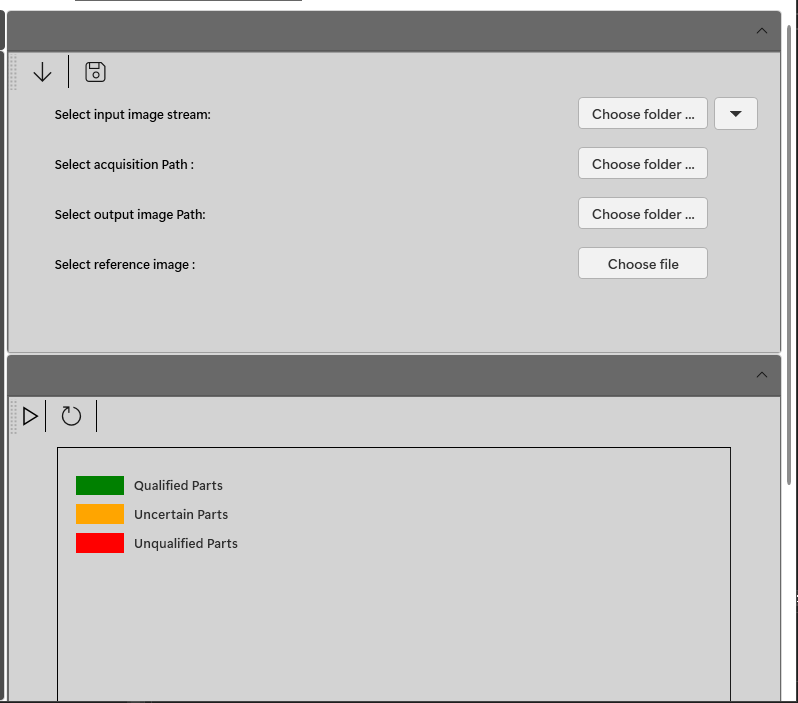
\includegraphics[height=8cm]{ressources/images/fenetre_disposition.png}
    \caption{la fenêtre principale}
\end{figure}

\section{Multiples modules pour PowerEye}
Après l'introduction générale du \texttt{PowerEye}, cette section va le présenter en détail à partir de chaque module.

\subsection{Préparation des données}
Le traitement des données étant une condition préalable à la formation au modèle, un module a également été spécialement conçu dans \texttt{PowerEye} pour mettre en œuvre les fonctions correspondantes. Dans ce module, nous avons actuellement développé deux interfaces entièrement fonctionnelles, à savoir l'extraction d'images et l'ajout du bruit de perlin. 
\subsubsection{Extraction d'images}
L'objectif de cette interface est d'extraire le contour de la pièce sur le photo de la ligne d'assemblage. Lorsque j'ai commencé à développer \texttt{PowerEye}, une fonction qui utilise le \texttt{feature matching} pour réaliser cet objectif a déjà été développée. Donc ma tâche principale a consisté à l'intégrer dans l'interface et à y apporter des améliorations. 

Lors de la conception de l'interface graphique pour cette fonctionnalité, j'ai suivi l'idée générale selon laquelle la partie supérieure de l'interface est utilisée pour la sélection de la configuration. Dans la partie inférieure de l'interface, j'ai conçu une barre de progression et une fenêtre pour montrer l'image avant et après le traitement. 
\begin{figure}[H]
    \centering
    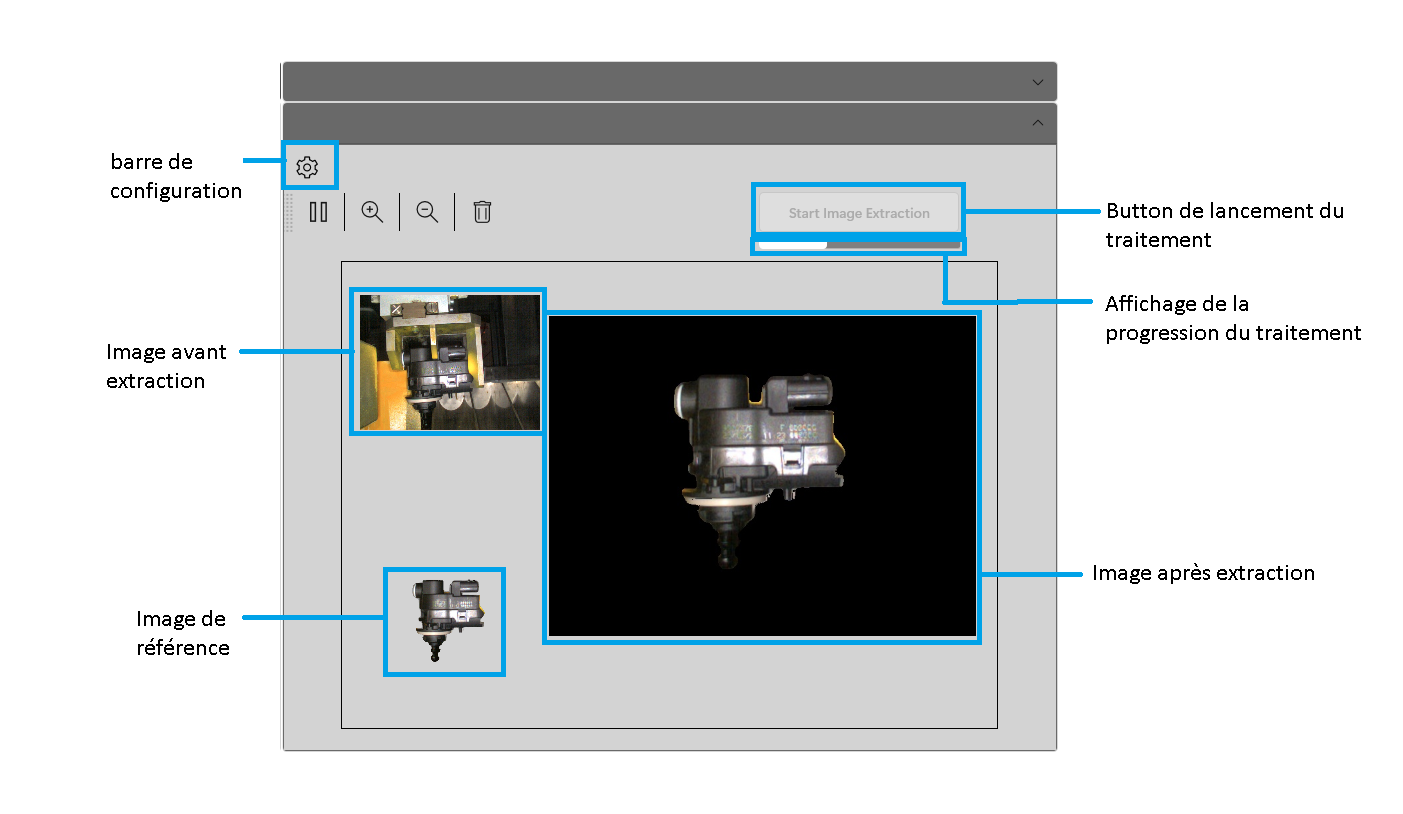
\includegraphics[height=8.5cm]{ressources/images/imageExtract.png}
    \caption{l'interface graphique d'extraction d'images}
\end{figure}

En ce qui concerne l'intégration de la fonctionnalité d'extraction développée, j'ai résolu deux problèmes principaux. D'une part, la fonction est développée en C++, tandis que l'interface est développée en C\#, il faut donc choisir la bonne méthode pour l'appeler. En final, j'ai choisi d'utiliser la même méthode que l'interface prototype, en appliquant le ficher \texttt{dll} pour l'importation et l'exportation des fonctions. D'autre part, c'est un problème très courant dans le développement d'interface graphiques est de savoir comment exécuter la fonction sans bloquer l'interface graphique. Donc le \texttt{thread} est utilisé pour résoudre ce problème. J'ai intégré la fonction extraite dans un \texttt{thread} et appliqué \texttt{FileWatcher} pour détecter les images ajoutée au répertoire afin de les afficher. Plus précisément, il fonctionne de la manière suivante : 
\begin{enumerate}
    \item Après de cliquer sur le bouton de démarrage, un nouveau \texttt{thread} est créé pour exécuter la fonction d'extraction d'image. 
    \item \texttt{FileWatcher} surveille toujours le répertoire de destination et détecte si les images traitées ajoutées sont occupées.
    \item Lorsque l'image n'est plus occupée, modifie le propriété de la source de liaison dans le \texttt{thread} principal pour l'afficher.
\end{enumerate}

\subsubsection{Ajout du bruit de perlin}
L'objectif de cette interface est d'ajouter un masque de bruit à l'image pour générer des pièces comportant des défauts. Comme dans la partie précédent, il existe déjà une fonction permettant d'ajouter des masques de bruit, développée à l'aide de python. L'idée de conception et la manière de fonctionner de cette partie sont similaires à la précédente, que je vais brièvement présenter ici. L'interface graphique est présentée comme ci-dessous. 
\begin{figure}[H]
    \centering
    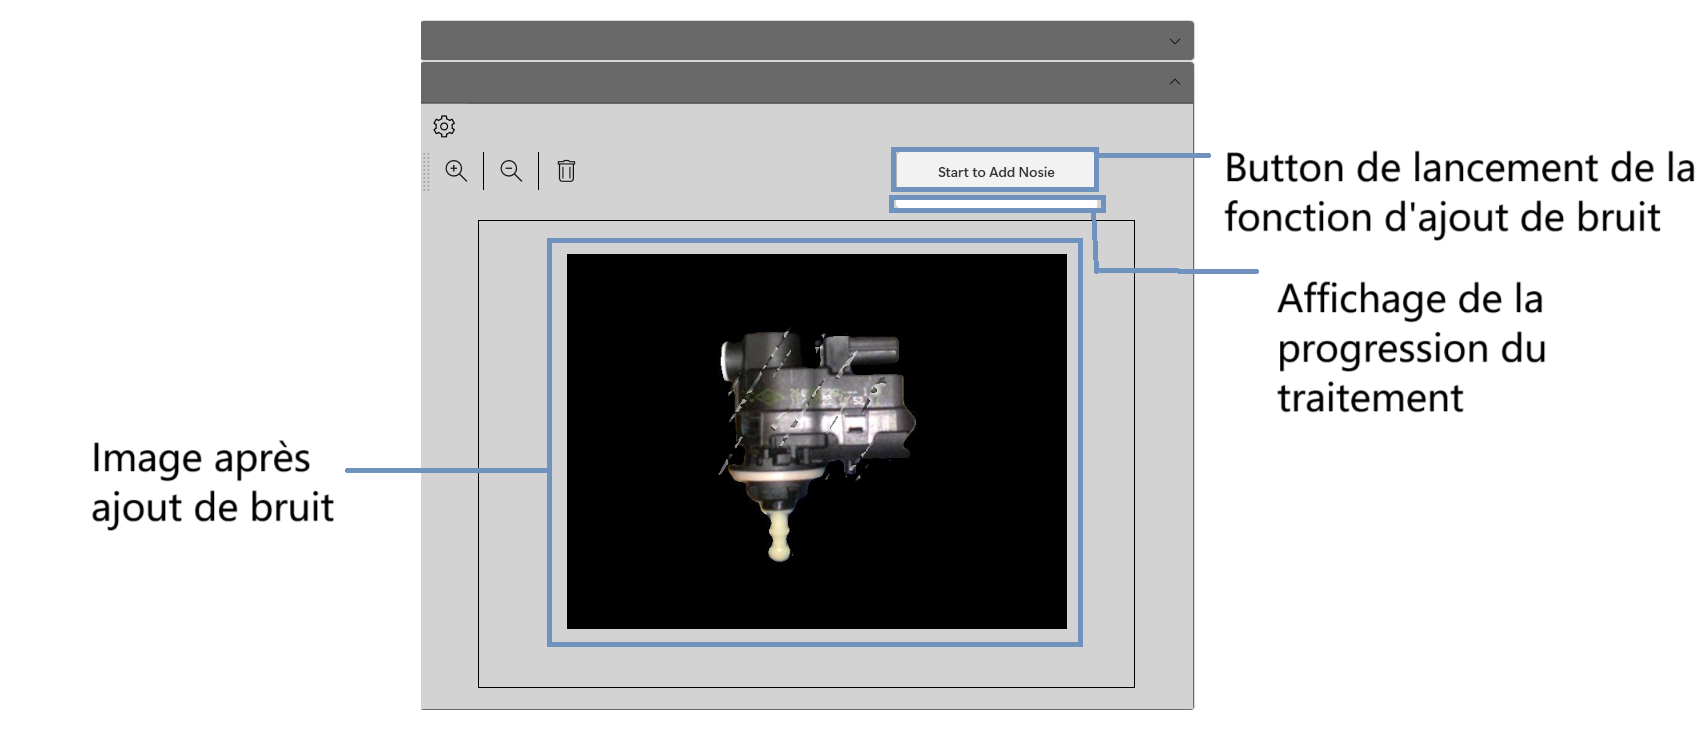
\includegraphics[height=8cm]{ressources/images/perlin_noise.png}
    \caption{l'interface graphique d'ajout du bruit}
\end{figure}

Et dans la section, je vais me concentrer sur la méthode d'appel python et sur une amélioration que j'ai réalisée. Pour l'appel au module python, je me réfère à l'implémentation de l'interface prototype. La classe \texttt{process} en C\# me permet d'exécuter python et de passer le script à lancer comme les paramètres de démarrage. Et dans la mise en œuvre, j'ai également encapsulé le processus python, y compris les valeurs d'entrée et de sortie, dans une classe pour le réutiliser dans le module d'apprentissage automatique. 

En termes d'améliorations, la fonction d'ajout de bruit nécessite trois paramètres d'entrée: une image de la pièce, un masque de bruit et un masque de forme. 
\begin{figure}[H]
    \centering
    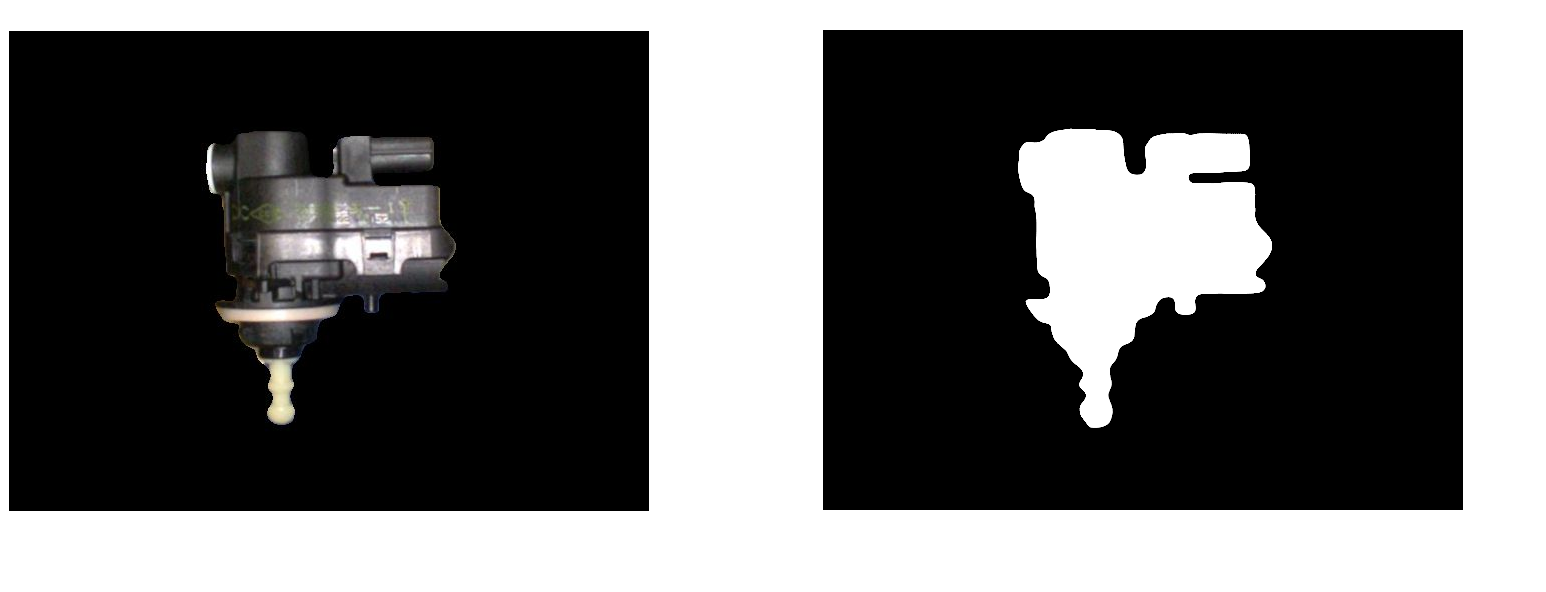
\includegraphics[height=4cm]{ressources/images/input_perlin.png}
    \caption{trois paramètres d'entrée}
\end{figure}
Mais en effet, il n'est pas difficile d'obtenir le masque de forme d'une pièce à partir de l'image initial. Par conséquent, j'ai développé la fonction pour générer les masques de forme afin de réduire la paramètre d'entrée. Les étapes pour réaliser cette fonction sont les suivantes: 
\begin{enumerate}
    \item Chargement et conversion de l'image d'entrée en niveaux de gris et Application d'un flou gaussien.
    \item Calcul de la magnitude et de la direction du gradient à l'aide de l'algorithme de Scharr.
    \item Normalisation de la magnitude du gradient dans la plage [0, 255].
    \item Opération de fermeture morphologique et recherche du plus grand contour d'arête.
    \item Générer et exporter des masques transparents avec des contours de remplissage maximaux.
\end{enumerate}

Après avoir terminé cette partie de l'amélioration, le module de préparation des données est désormais plus robuste, ce qui permet de passer au module d'apprentissage automatique qui utilise les données.

\subsection{Apprentissage automatique}


\subsection{Contrôle de la chaîne d'assemblage} 
Ce module, qui est l'application la plus importante de tout le logiciel, permet de détecter les images des pièces sur la ligne d'assemblage et de sauvegarder les données.

\subsubsection{Surveillance de la ligne d'assemblage}
L'idée de cette fonction est d'utiliser le modèle entraîné pour inspecter chaque image de pièce et d'afficher les résultats de l'inspection dans l'interface. Mais pendant le développement, il était impossible d'accéder aux capteurs dans la scène réelle. J'ai donc utilisé un processus qui copie les images dans un répertoire toutes les cinq secondes comme une alternative. 

Dans la conception de l'interface, j'ai choisi d'utiliser différentes couleurs pour indiquer si le pièce est qualifiée ou non, un peu comme le voyant d'avertissement, et afficher l'image de ce pièce. L'interface graphique conçue est illustrée ci-dessous.
\begin{figure}[H]
    \centering
    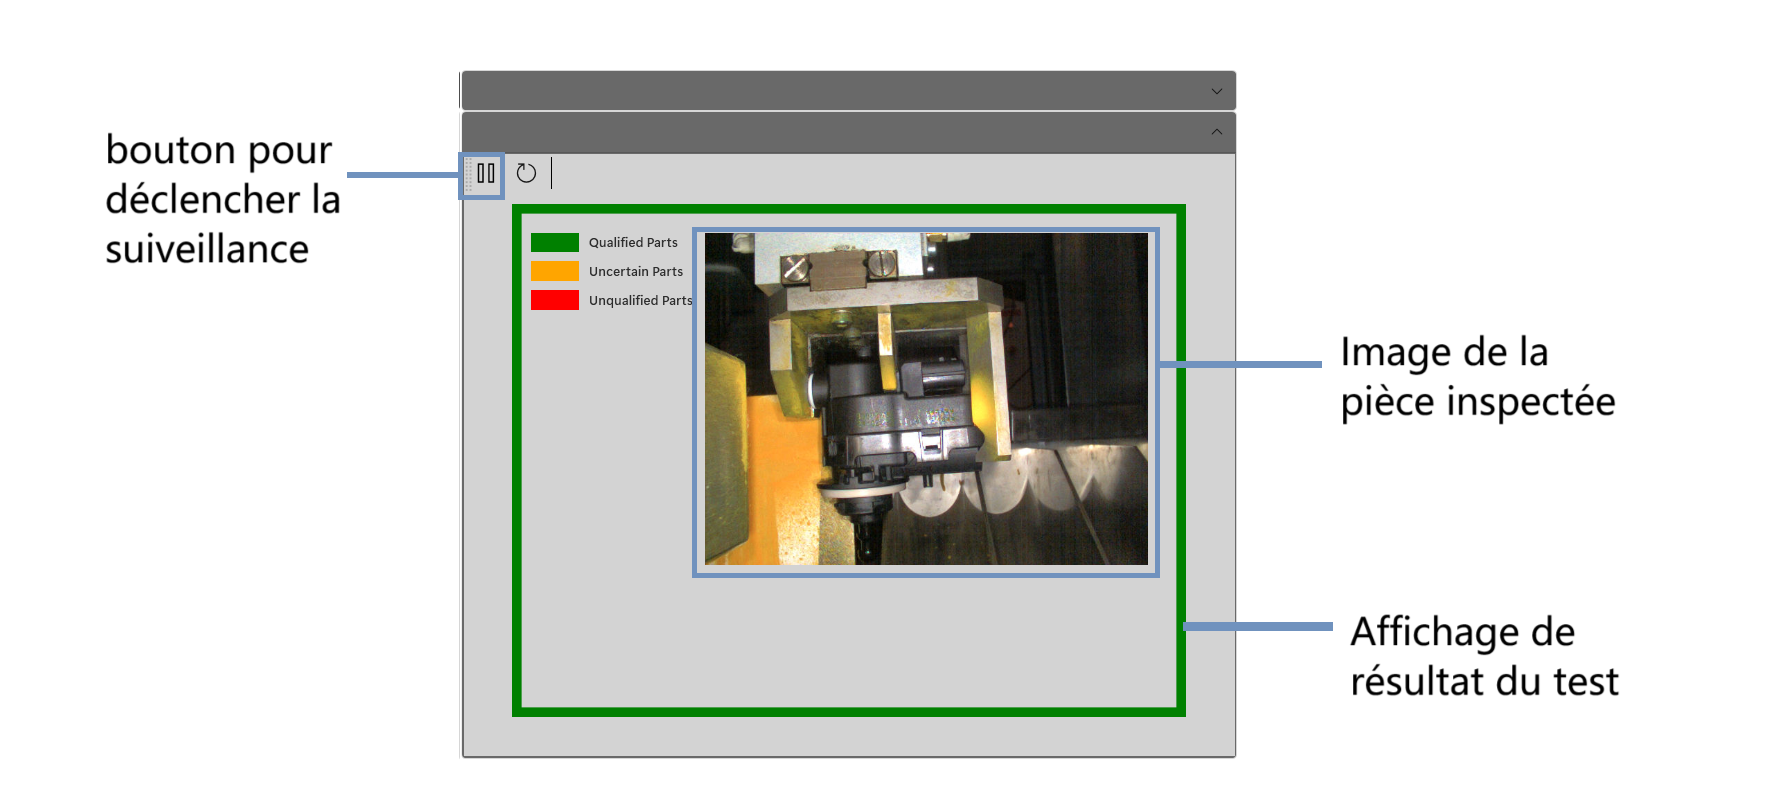
\includegraphics[height=8cm]{ressources/images/monitoring.png}
    \caption{Interface graphique de la surveillance de la ligne d'assemblage}
\end{figure}

 Les pièces dont le score est inférieur à 90 sont considérées comme non qualifiées, celles dont le score est supérieur ou égal à 95 sont considérées comme qualifiées, et celles dont le score est compris entre 90 et 95 doivent être testées à nouveau manuellement. La réalisation de la fonctionnalité utilise la même approche que dans la section précédente, en utilisant  un \texttt{thread} et \texttt{FileWathcer} pour assurer l'interaction de l'interface.

\subsubsection{Sauvegarde des données de pièces}
Une fois la pièce analysée, ses données sont sauvegardées dans une autre interface. Dans cette interface, j'ai conçu trois listes pour stocker les données des différents types de pièces, y compris son temps de production, le nombre de points gagnés et le chemin où l'image est sauvegardée. 
\begin{figure}[H]
    \centering
    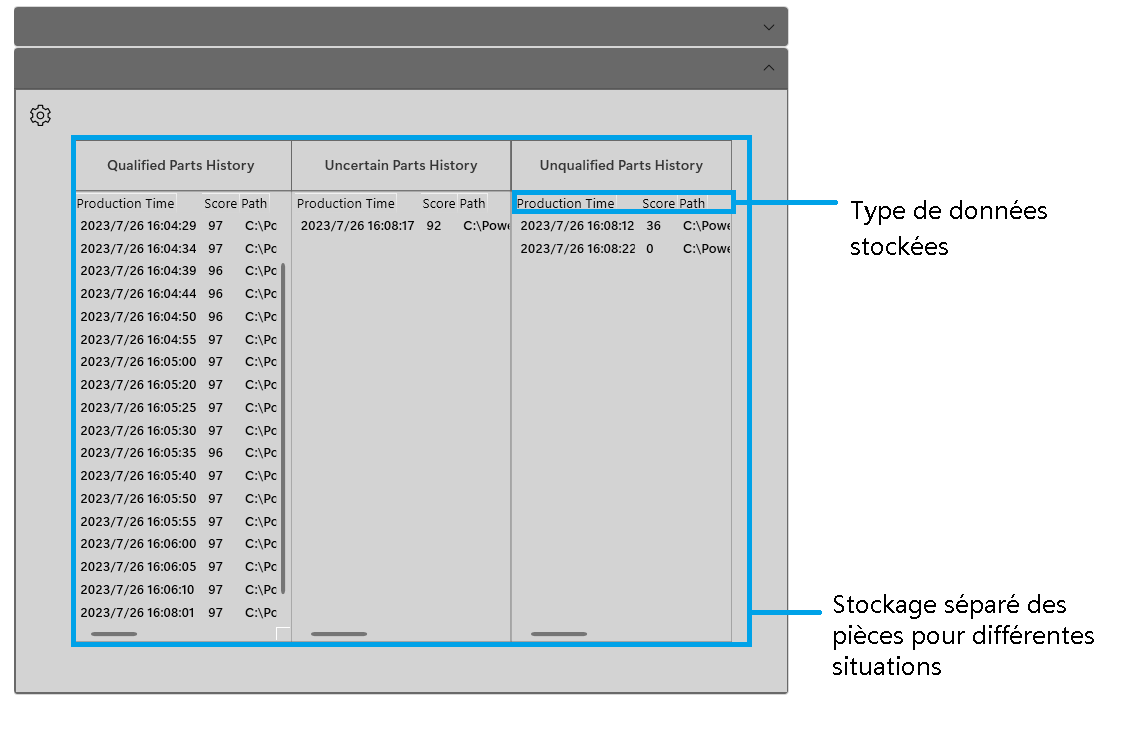
\includegraphics[height=8cm]{ressources/images/check_parts.png}
    \caption{Interface graphique pour le stockage des données relatives aux pièces }
\end{figure}

Et pour les pièces dont la qualification n'est pas certaine, vous pouvez les vérifier manuellement en cliquant sur la liste. Une nouvelle fenêtre apparaît alors et l'état de la pièce peut être vérifié en faisant glisser l'image vers la gauche ou la droite. 
\begin{figure}[H]
    \centering
    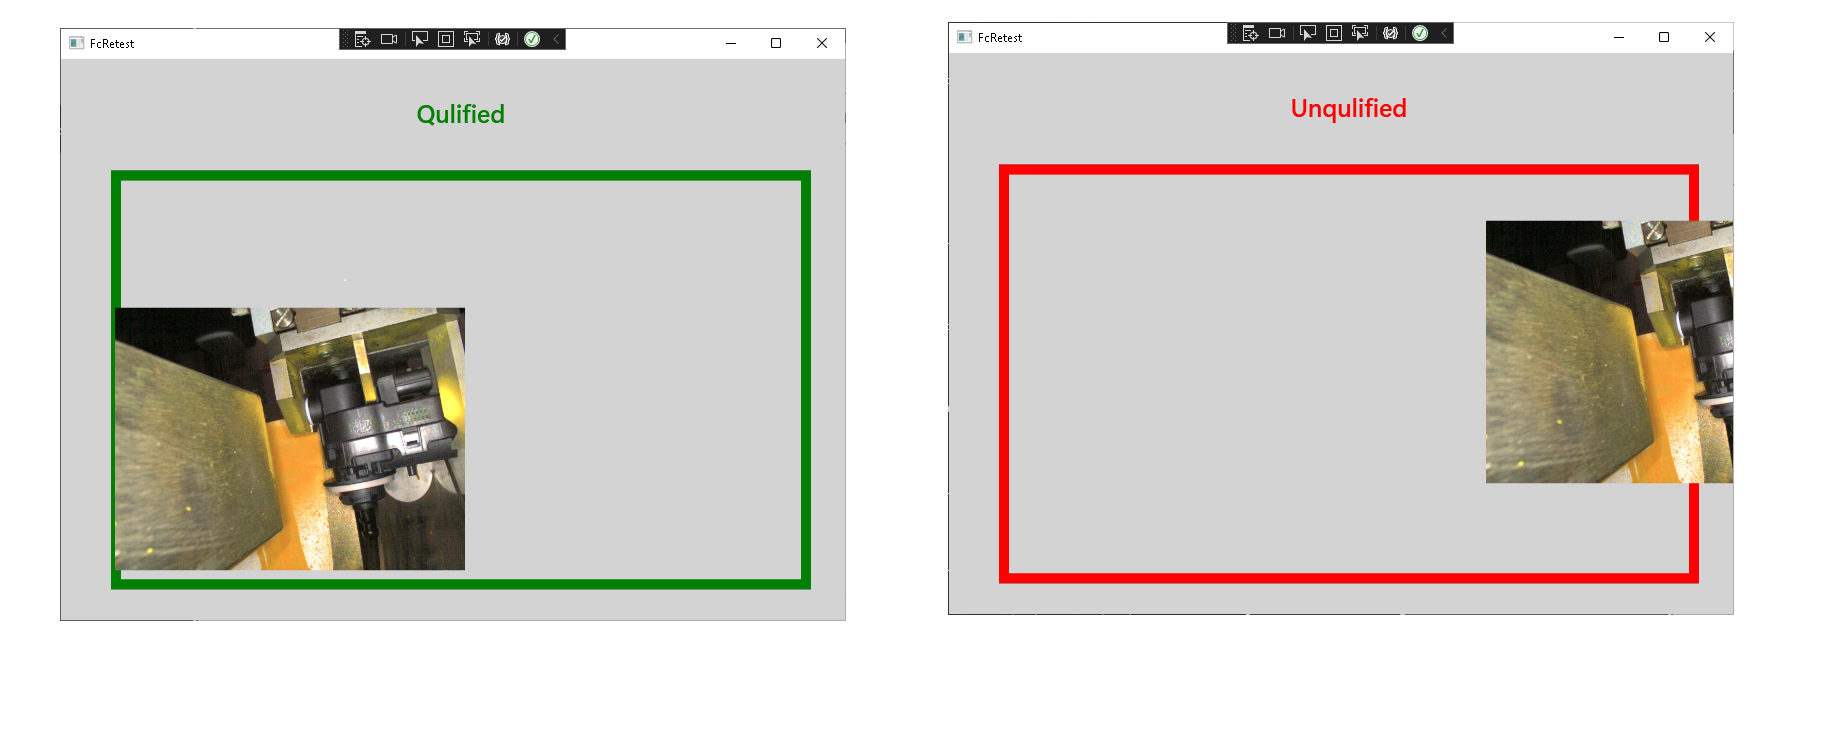
\includegraphics[height=6cm]{ressources/images/check_manuel.png}
    \caption{Interface graphique pour la vérification manuelles}
\end{figure}

\subsection{Suivi des données relatives aux pièces}
Le module est conçu pour une utilisation à long terme et retracer les données de la pièce précédente enregistrées dans des fichiers \gls{Excel}. 

\subsubsection{Interroger les données historiques}
L'idée de cette fonction est d'afficher le fichier \gls{Excel} sélectionné dans l'interface, d'effectuer une recherche par mot-clé et d'enregistrer les résultats de la recherche. 

Dans la conception de l'interface, J'utilise une grille de données pour afficher les données d'un fichier \gls{Excel}, une barre de sélection pour choisir le type de données à filtrer et une zone de texte pour saisir des mots-clés. 
\begin{figure}[H]
    \centering
    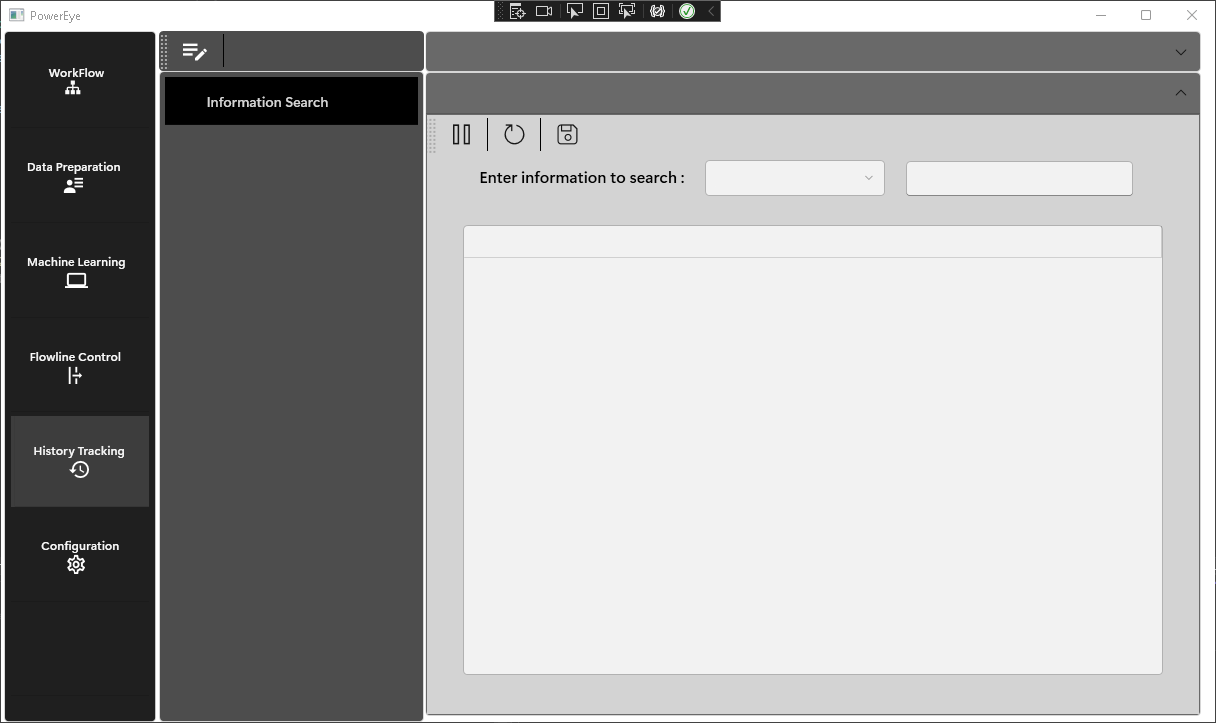
\includegraphics[height=9cm]{ressources/images/information_search.png}
    \caption{Interface graphique pour l'interrogation de l'historique }
\end{figure}

Afin de lire le fichier Excel, une extension \texttt{ClosedXML} est utilisée, ce qui me permet d'obtenir le contenu du fichier par chemin et de le stocker dans la classe \texttt{DataTable}.  J'ai ainsi créé deux fonctions pour convertir un chemin d'accès en \texttt{DataView} contenant un tableau et un chemin d'accès en une liste contenant les lignes d'en-tête d'un tableau. Et pour obtenir cette fonction de filtrage, la propriété \texttt{RowFilter} de \texttt{DataView} est tout à fait appropriée, il suffit de changer sa valeur en fonction de différents mots-clés pour modifier le contenu de l'affichage. Enfin, pour pouvoir enregistrer le tableau filtrée, il est nécessaire de créer une classe \texttt{DataView} qui supprime effectivement les données en fonction du \texttt{RowFilter} et de la convertir en utilisant l'extension. 

\subsection{Configuration des données globales}
Le module est principalement conçu pour permettre aux développeurs de compléter la sélection de la configuration de plusieurs modules directement par l'importation de fichiers de configuration afin de faciliter les tests. Par ailleurs, dans les scénarios d'application pratique, la construction de l'environnement d'exécution peut également être facilitée par une configuration globale.

\subsubsection{Affichage des informations sur la configuration actuelle}
L'interface est conçue pour permettre aux développeurs de visualiser la configuration globale actuelle du logiciel. Dans la section précédente de l'introduction générale, j'ai expliqué la structure de données qui compose \texttt{PowerEye}, consistant en les listes d'exemples de composants pour chaque interface de chaque module. Je n'ai donc besoin que d'afficher cette classe de données sur l'interface. Dans le choix de la méthode, j'ai choisi d'afficher le contenu après la sérialisation \gls{XML}, car cela convient mieux à ma réalisation ultérieure de la fonction d'importation et d'exportation, d'autre part, c'est plus pratique que de reconstruire toute la fonction \texttt{tostring} de données. En outre, j'ai développé la fonctionnalité de sérialisation afin de sauvegarder les configurations actuelles. 

En termes de conception de l'interface graphique, cette section est plutôt simple, avec une zone de texte pour afficher les informations de configuration et un bouton pour sauvegarder la configuration actuelle.
\begin{figure}[H]
    \centering
    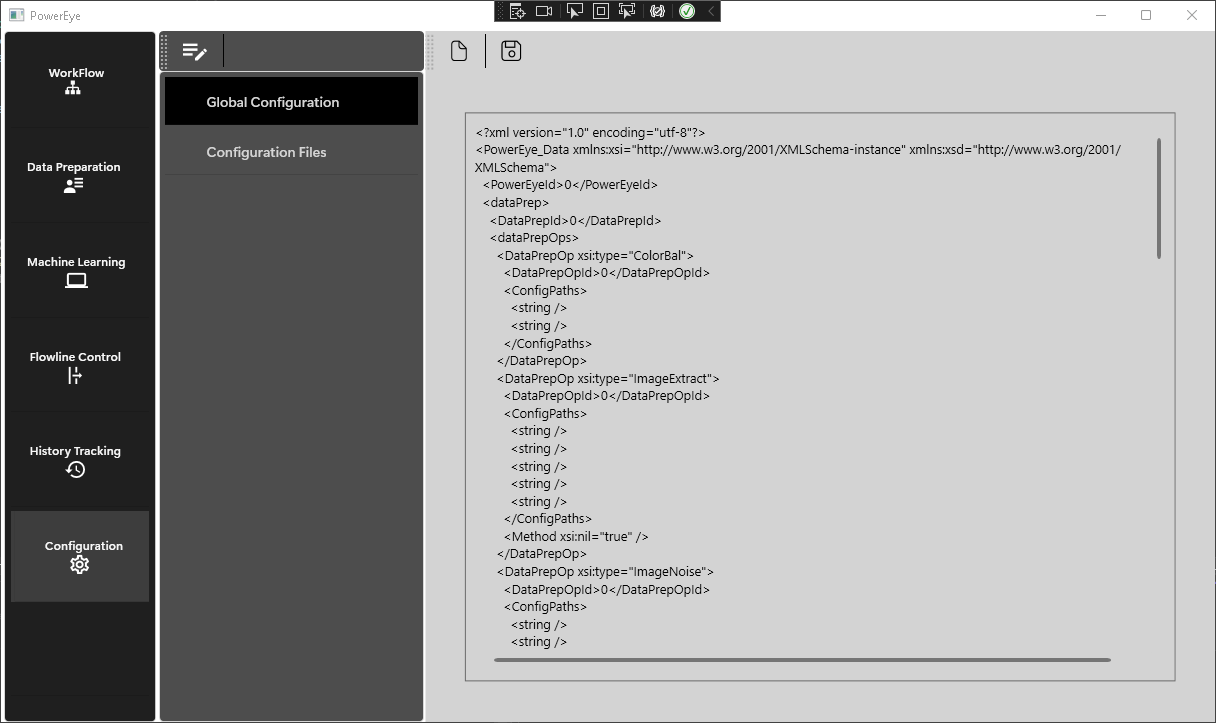
\includegraphics[height=8cm]{ressources/images/global_configuration.png}
    \caption{Interface graphique montrant la configuration globale}
\end{figure}

\subsubsection{Importation de configuration}
Cette interface est conçue pour appliquer les configurations précédemment sauvegardées à l'ordinateur. En utilisant la désérialisation \gls{XML}, nous pouvons reconstruire le fichier sauvegardé en classe de données de \texttt{PowerEye}. Dans la classe de données, j'ai implémenté une fonction de copie pour chaque sous-classe afin de remplacer la valeur par la valeur générée par le fichier. 


\begin{figure}[H]
    \centering
    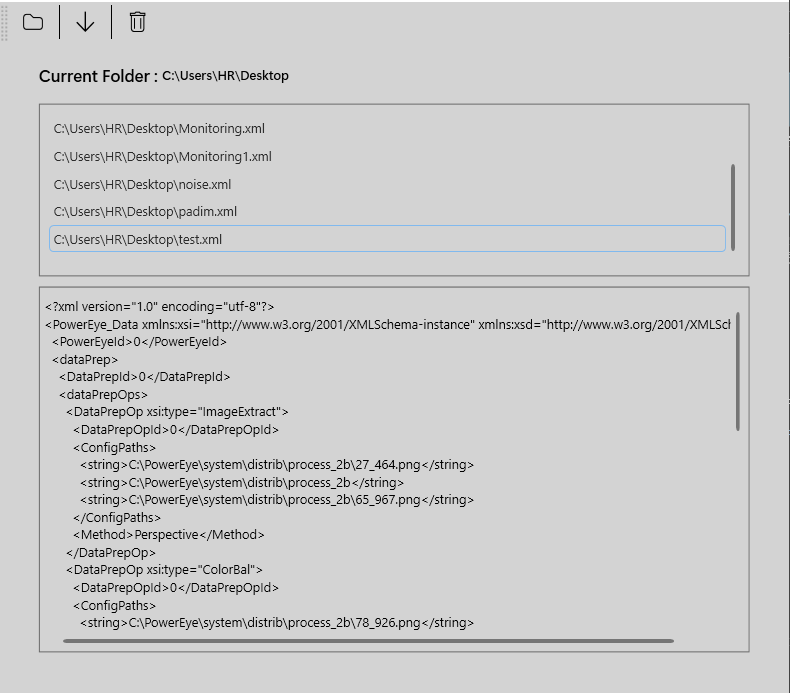
\includegraphics[height=8cm]{ressources/images/configuration_files.png}
    \caption{Interface graphique montrant la configuration globale}
\end{figure}









\subsection{Flux de travail personnalisés}
\section{Fonctions en dehors du corps principal}
Dans le dernière partie de mes réalisations, je vais présenter deux fonctionnalités que j'ai développées en dehors du corps principal du logiciel. Bien que ces deux fonctions ne constituent pas directement le logiciel, elles contribuent au processus de tests.
\subsection{Affichage de l'appel de fonction}
\begin{figure}[H]
    \centering
    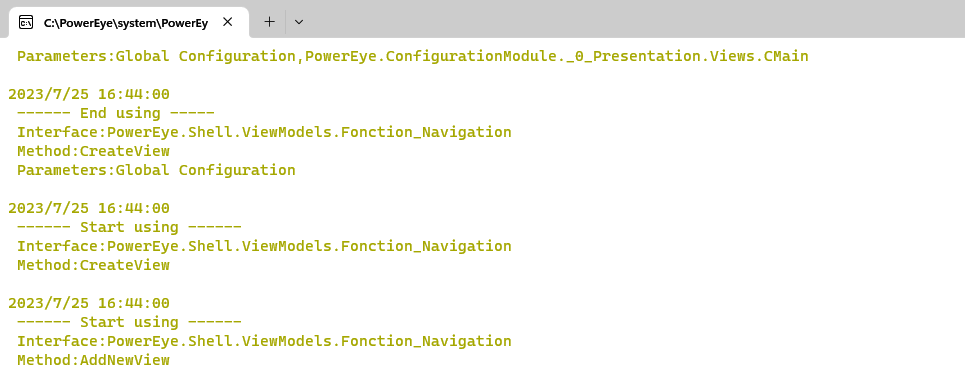
\includegraphics[height=7cm]{ressources/images/aop_log.png}
    \caption{l'interface graphique d'ajout du bruit}
\end{figure}
\subsection{Exécution de la chaîne de caractères comme un script}

